% IEEE PAPER FORMAT 
\documentclass[twocolumn,oneside,conference]
{IEEEtran}

%%%%%%% all the required packages are loaded%%%%
\usepackage{filecontents}
\usepackage[style=ieee,backend=biber]{biblatex}
\usepackage{graphicx}
\usepackage{lmodern}
\usepackage{enumerate}
\usepackage{float}

% bibilography page%%%%%%%%%%%%%%
\begin{filecontents}{Master.bib}
@proceedings{this123,
editor = {Sriharsha Harsha et al},
title = {This is a test paper},
year = {2016}
}
\end{filecontents}
%%%%%%%%%%%%%%%%%%%%%%%%%%%%%%%%%%%%%%%



\addbibresource{Master.bib}

\IEEEoverridecommandlockouts 
\renewcommand\IEEEkeywordsname{Keywords}


\title{ICNV-TV: A read-depth based Copy Number Variation detection tool}
\markboth{Journal of Not yet Decided}{Sriharsha \MakeLowercase{\textit{et al}}: A read-depth based Copy Number Variation detection tool}

\author{
	\IEEEauthorblockN{Sriharsha Vogeti} 
	\IEEEauthorblockA{CCNSB,IIIT-Hyderabad\\
	vogetisri.harsha@research.iiit.ac.in}
	\and
	\IEEEauthorblockN{Prashanthi D} 
	\IEEEauthorblockA{CCNSB,IIIT-Hyderabad\\
	prashanthi.d@research.iiit.ac.in}
	\and
	\IEEEauthorblockN{Nita Parekh} 
	\IEEEauthorblockA{CCNSB, IIIT-Hyderabad\\
	nita@iiit.ac.in}
	
}

\begin{document}
\maketitle


 
\begin{abstract}
These instructions provide basic guidelines for preparing camera-ready (CR)
Proceedings-style papers. This document is itself an example of the
desired layout for CR papers (inclusive of this abstract). The document
contains information regarding desktop publishing format, type sizes, and
type faces. Style rules are provided that explain how to handle equations,
units, figures, tables, references, abbreviations, and acronyms. Sections
are also devoted to the preparation of the references and acknowledgments.\\
\end{abstract}

\begin{IEEEkeywords}
CNV Detection, CNVTV, Read-Depth Methods, Population Studies, NGS\\
\end{IEEEkeywords}
\section{Introduction}
\IEEEPARstart{S}ome shit \cite{this123}

\section{Methods}
General input description 
\subsection{Preprocessing}
\subsection{Segmentation}
\subsection{Postprocessing}

\section{Results}
Discussion about what has been done
\subsection{Simulated Data}
\subsection{Real Data Analysis}
\subsection{Sub-population Analysis}
\begin{figure*}[h]
	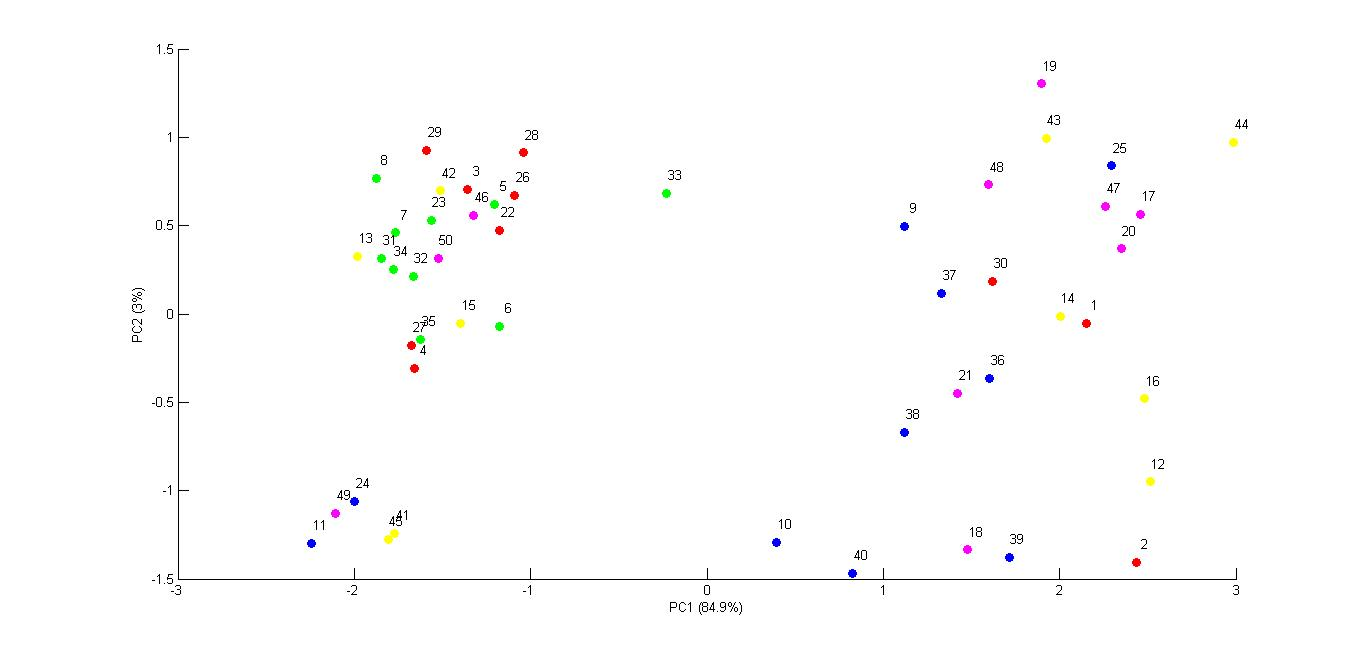
\includegraphics[width=\linewidth]{final.jpg}
	\caption{This is a test image}
	\label{fig1: this is test image}
\end{figure*}

\section{Discussion}

\section{Future work}

\section*{Acknowledgments}


\printbibliography

\end{document}



